
% Chapter 1 - Introduction 
% ------------------------
% Jun 6, 2015


\chapter{Introduction}

\section{Dissertation outline}

\noindent
This dissertation is organized into four chapters. Each chapter was designed as a self-contained work to address the specific objectives proposed in this PhD research (below). {\sl Chapter~1} presents an introduction to the scientific questions being addressed and the background needed to follow the work developed in {\sl Chapters 2--4}. {\sl Chapter~2} describes the full method implemented in this study (partially developed and partially modified from previous work) to construct the longest, continuous and high-resolution (in time and space) time series of changes in ice-shelf surface-height from multiple satellite radar altimeters (RAs). In this chapter, the RA data and corrections are discussed, and new processing approaches are proposed. This chapter is in revision for the journal {\it Remote Sensing of Environment}. {\sl Chapter~3} describes the trend analysis approach implemented in the ice-shelf height time-series product (derived in {\sl Chapter~2}), as well as reporting and discussing some of the main findings of this dissertation, which have significantly advanced our understanding on the state of the Antarctic ice shelves. This chapter was published in the journal {\it Science}. {\sl Chapter~4} focuses on the variability analysis of the ice-shelf height time series. This chapter investigates the origin of interannual fluctuations in ice-shelf thickness, and seeks to understand the links between observed ice-shelf changes and large-scale climate variability. The material in this chapter is currently being prepared for publication.


\section{Antarctic ice sheet, ice shelves and sea-level change}

\noindent
The Antarctic Ice Sheet gains mass through snowfall and loses mass through submarine melting and iceberg calving of its ice shelves, the marginal floating extensions of inland glaciers and ice streams. Both these processes, melting and calving, contribute about the same to ice-shelf loss \parencite{Rignot2013, Depoorter2013}. More than 80\% of Antarctica's ice drains through these ice shelves, where most of the mass
lost from the ice sheet is transferred to the ocean (Fig.~\ref{fig:ice-sheet-flow}). The Antarctic Ice Sheet contains ice equivalent to $\sim$58 m of global sea-level rise\footnote{A moderate loss of 2\% of the Antarctic Ice Sheet is sufficient to rise
global sea level by $\sim$1 m.} \parencite{Fretwell2013}, and has been losing mass at an average rate of
$\sim$71 Gt year$^{-1}$ (gigatonnes per year)\footnote{360 Gt of ice corresponds roughly to 1 mm of sea-level rise.} between 1992 and 2011
\parencite{Shepherd2012}. This is equivalent to a contribution of
(slightly over) 6\% to the total sea-level rise of $\sim$3.2 mm year$^{-1}$.
 More important than the current (small) contribution to sea-level rise, however, is the accelerated state of this ice-loss rate, as has been observed during the past decade \parencite{Shepherd2012, Sutterley2014, Velicogna2009, Chen2009, Harig2015}, which raises significant concern on future ice-sheet behaviour and its contribution to sea-level change. 


\begin{figure}[!ht]
  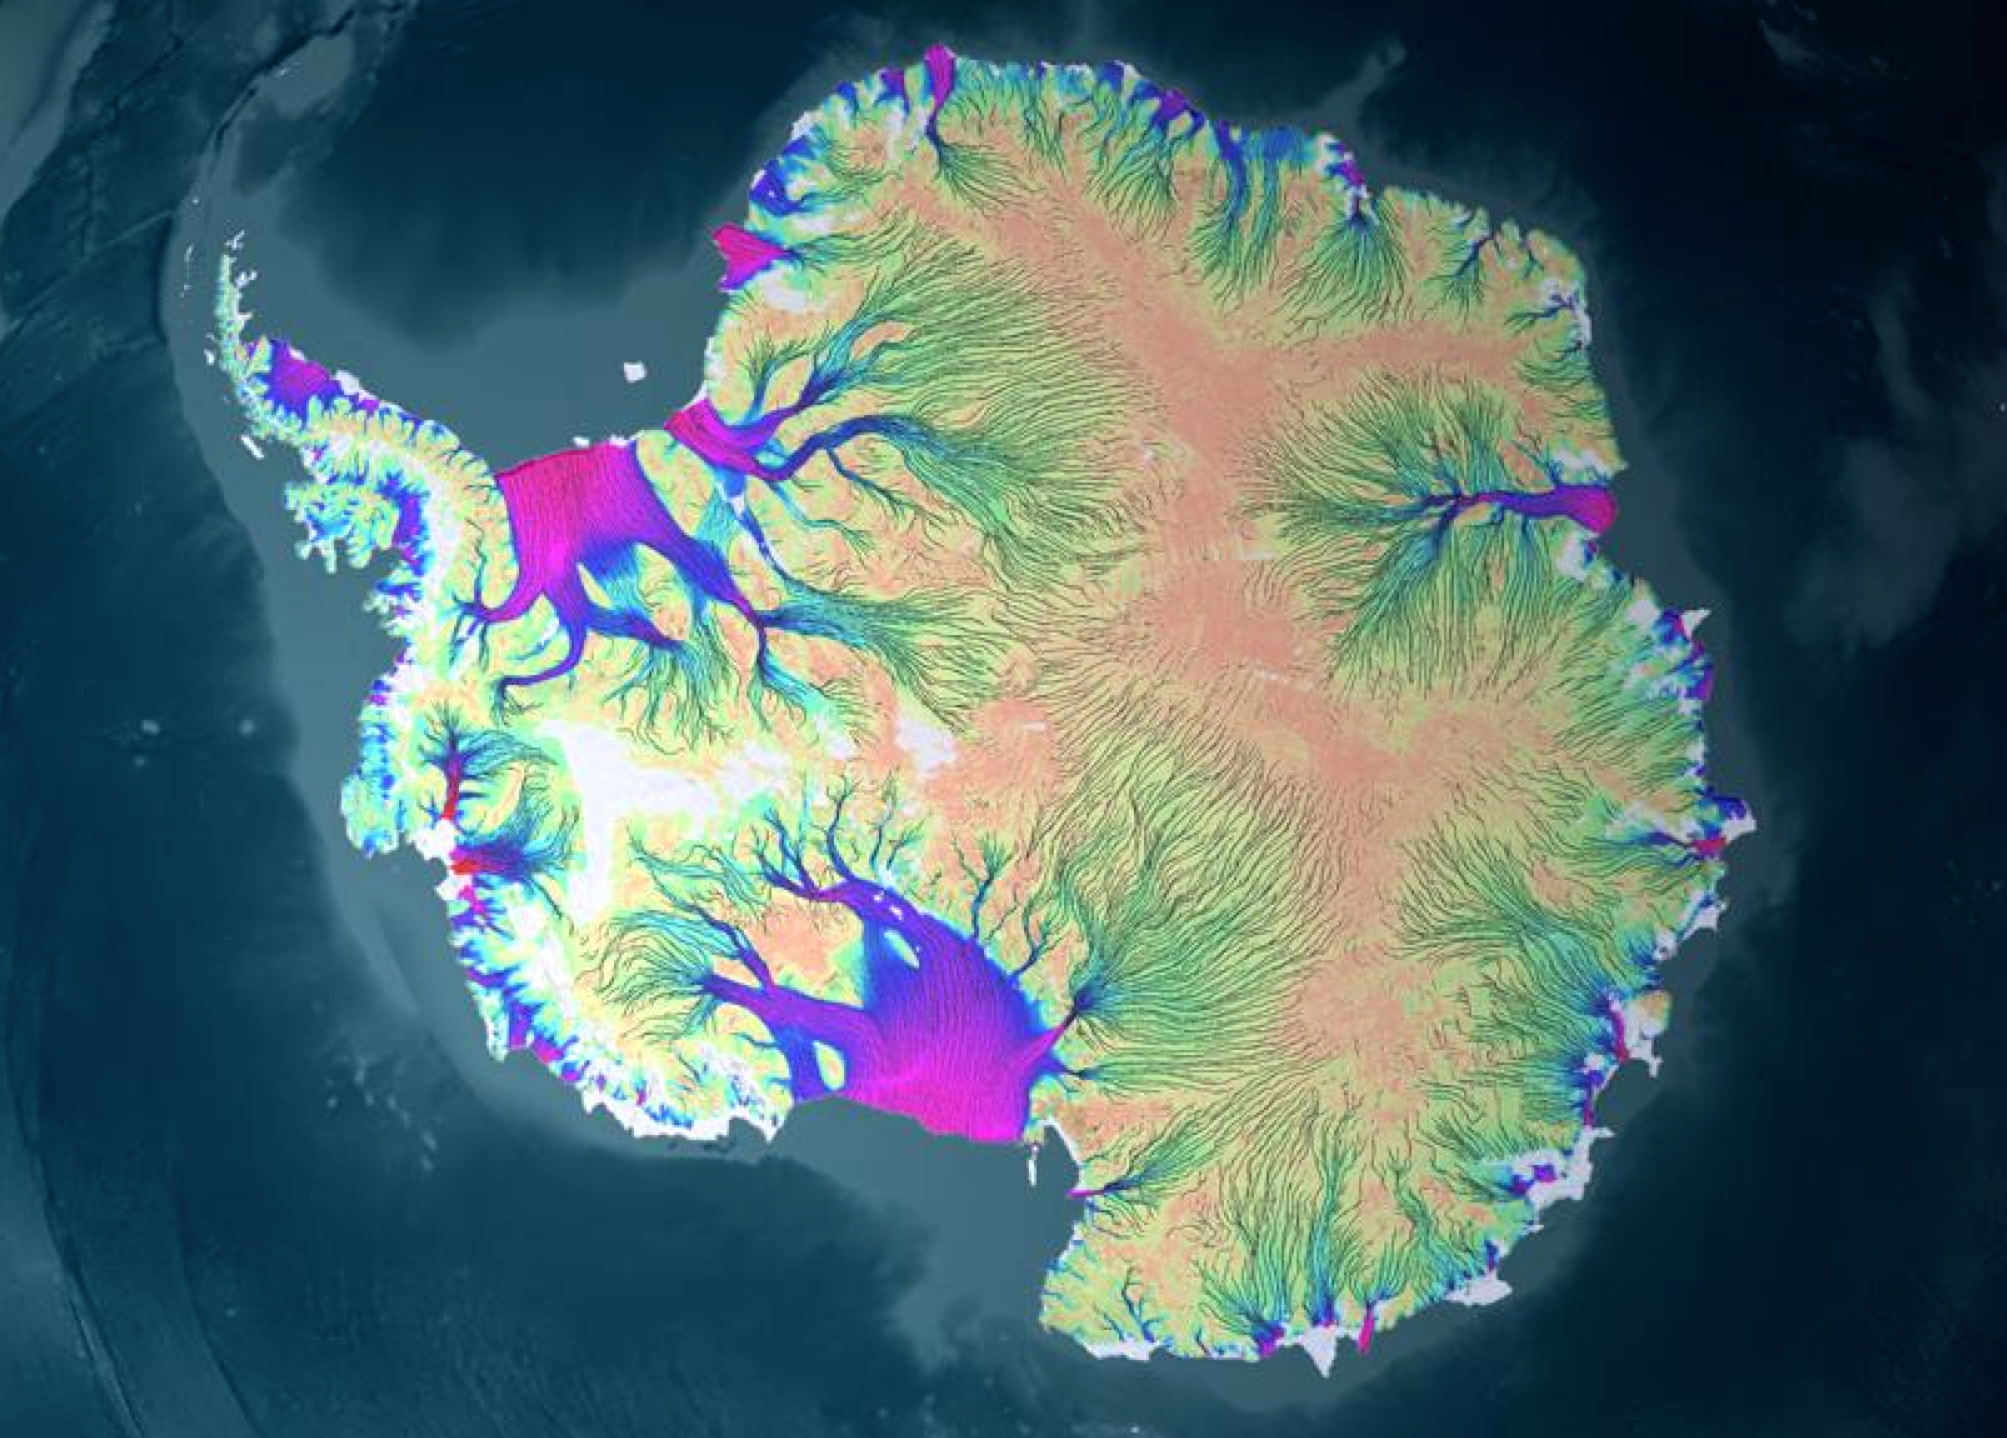
\includegraphics[width=\textwidth]{img/ice_sheet_flow2.png} % 2 | 3
  \caption[Ice flow of the Antarctic Ice Sheet]{
  Ice flow of the Antarctic Ice Sheet. Color map represents the horizontal velocity field of the ice-sheet's surface (orange is near-zero velocity and purple is maximum velocity), as derived from Interferometric Synthetic Aperture Radar (InSAR). The pattern shows ice flowing from the (inland) catchment basins towards the ocean through the fringing ice shelves, where flow speed is highest. {\it Credit: NASA; \textcite{Rignot2011}.}
  }
  \label{fig:ice-sheet-flow}
\end{figure}


Located at the boundary between the ice sheet, atmosphere and ocean,
Antarctica's ice shelves are potentially vulnerable to changes in both
atmospheric and oceanic conditions (Fig.~\ref{fig:ice-sheet-configuration}, making them sensitive indicators of
large-scale climate change. For more than two decades, rapid
changes have been occurring in the extent and thickness of many Antarctic ice
shelves, particularly along the Antarctic Peninsula and the Amundsen Sea
sector of West Antarctica \parencite{Cook2010, Pritchard2012, Shepherd2010,
Wingham2009, Zwally2005, Fricker2012}. It is,
therefore, through the ice shelves that variations in
oceanic and atmospheric states are "felt" by the ice sheet, as forcing mechanisms
to grounded-ice change.


\begin{figure}[!ht]
  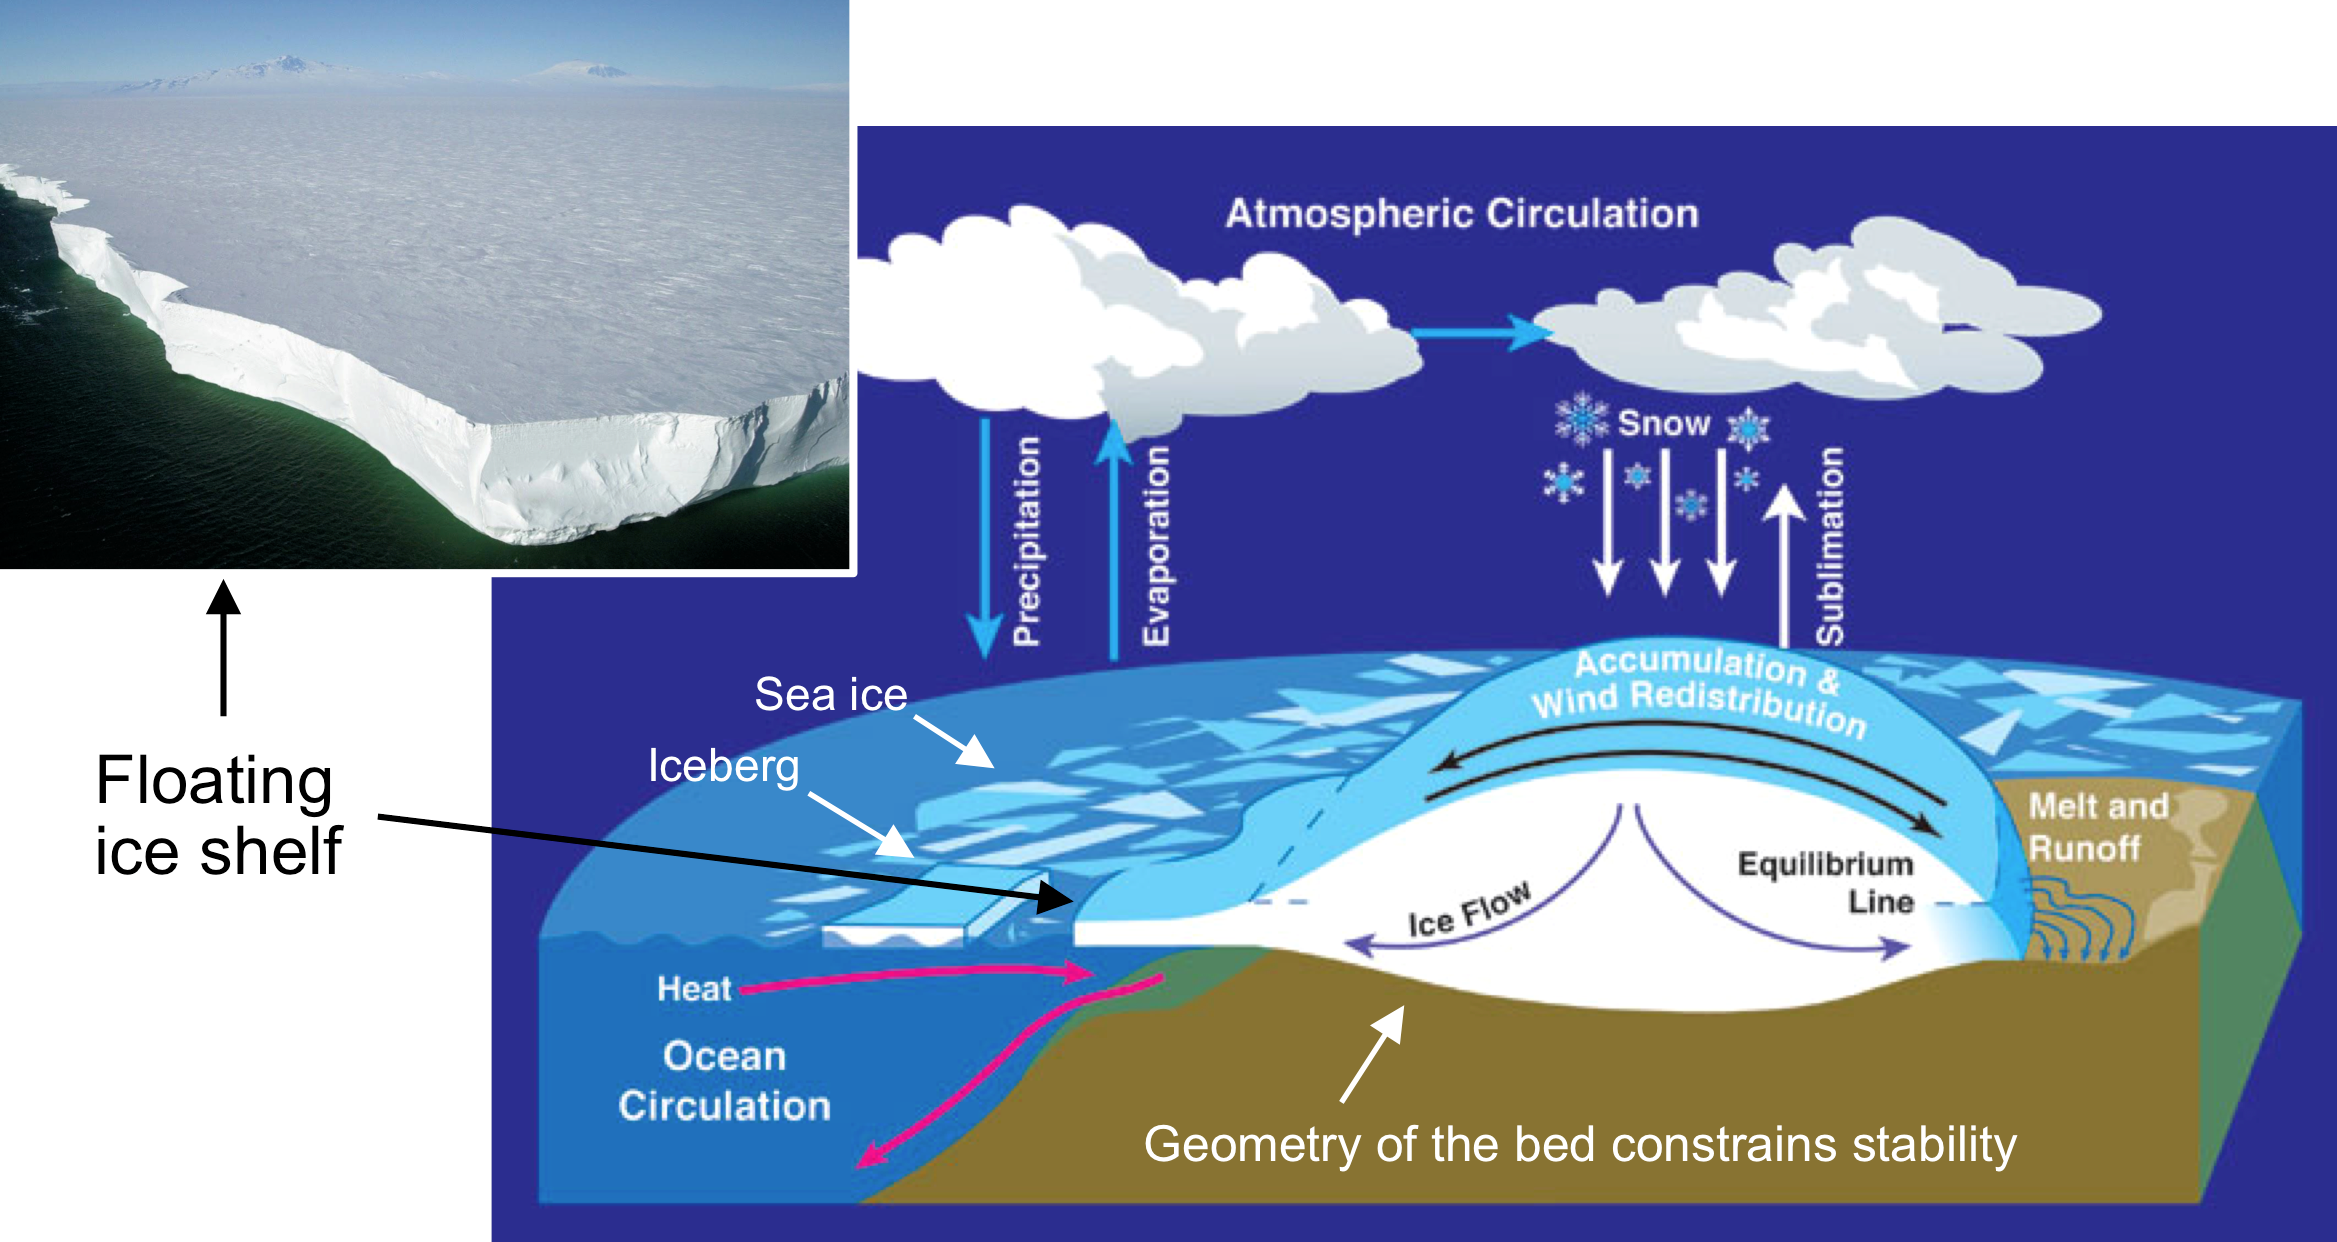
\includegraphics[width=\textwidth]{img/ice_sheet_configuration2.png} % 1 | 2
  \caption[Configuration of the Antarctic Ice Sheet]{
  Configuration of an ice sheet and the interaction with its surrounding ocean and atmosphere. The left hand side of the ice sheet depicts the characteristic configuration of the Antarctic Ice Sheet, while the right hand side is more characteristic of the Greenland Ice Sheet. Note that $\sim$90\% of all ice shelves are in Antarctica. {\it Credit: NASA}.
  }
  \label{fig:ice-sheet-configuration}
\end{figure}


In the past decade, considerable progress has been made in understanding the
fundamental role that ice shelves play in restraining the grounded ice-sheet
flow \parencite[e.g.,][]{Schoof2007, Goldberg2009, Gudmundsson2013}. Ice shelves exert a back-stress on grounded tributary-glaciers and ice streams resulting from drag forces
at the ice-bedrock interface. This resistive stress, known as the \emph{buttressing effect},
holds back the ice flow from the ice-sheet interior to the ocean (Fig.~\ref{fig:ice-shelf-buttressing}).
With loss of back-stress due to ice-shelf shrinkage or breakup, ice discharge
increases with grounding line (GL)\footnote{The grounding line
is the dynamic boundary between the grounded ice sheet and the floating ice shelves;
where glaciers/ice streams detach from the bedrock and start to float.} thickness (scaling nonlinearly) to
compensate for the reduction in \emph{buttressing} \parencite{Schoof2007, Joughin2012}. This nonlinear dynamics,
flow~$\propto$~thickness$^{n \geqslant 3}$ (at the GL), becomes particularly important in
regions where (a) the ice sheet is
grounded below sea level (marine ice sheet) and (b) the bed deepens inwards
(retrograde bed slope) (Fig.~\ref{fig:ice-sheet-configuration}). Such configuration gives rise to a condition of unstable
equilibrium known as the \emph{marine ice-sheet instability},
first proposed in the 1970s by, e.g., \textcite{Weertman1974, Mercer1978}.


\begin{figure}[!ht]
  \centering
  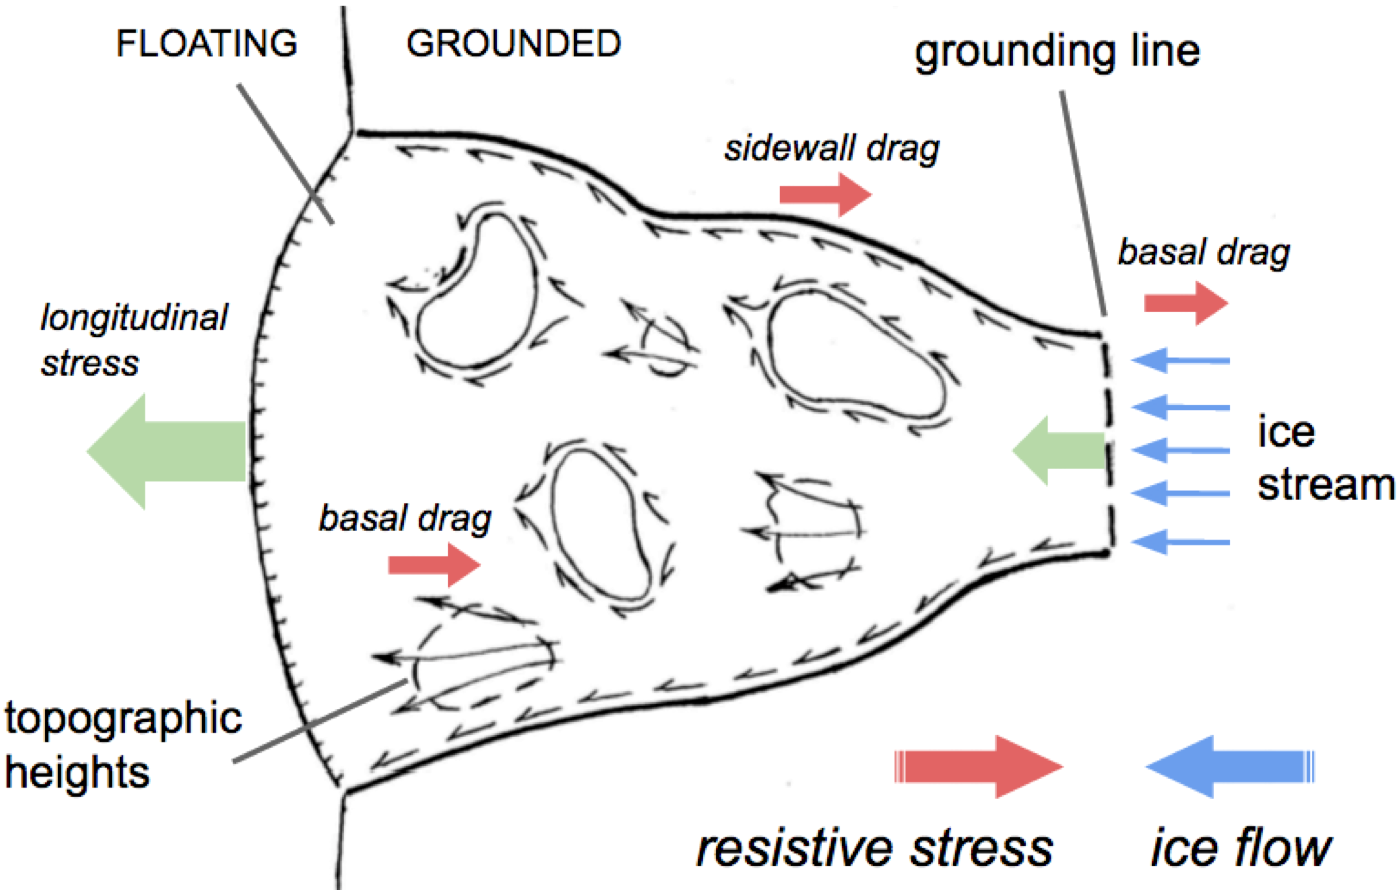
\includegraphics[width=.9\textwidth]{img/ice_shelf_buttressing.png}
  \caption[Schematic of ice-shelf buttressing]{
  Configuration of the ice-shelf/ice-sheet interaction. The arrows show the various forces that interplay at the ice-shelf/ice-sheet transition, giving rise to the buttressing effect (ice-shelf's ability to restrain the grounded ice-sheet flow). {\it Credit: modified from \textcite{Hughes2014}}.
  }
  \label{fig:ice-shelf-buttressing}
\end{figure}


There have been recent rapid advances in identifying the dynamical processes by which the
ocean can control ice-sheet mass loss and associated sea-level change (Fig.~\ref{fig:ice-shelf-schematic}). Studies have shown that
increased ocean-forced basal melting of ice shelves, leading to flow acceleration of adjacent grounded ice,
is responsible for the majority of current Antarctic ice sheet loss \parencite{Rignot2008,
Pritchard2009}. Dramatic grounding line retreat as a consequence
of intensified basal melting has induced extensive land ice thinning \parencite{Wingham2009,
Pritchard2009, Rignot2014}, and faster flow rates have followed ice shelf collapses
due to the reduction in buttressing \parencite{Rignot2004, Scambos2004}.
In fact, 87\% of all Antarctic Peninsula (AP) tidewater glaciers are known to be retreating
\parencite{Cook2005}, and dynamic thinning (increased strain rates due to flow acceleration)
has occurred around the AP \parencite{Rignot2008, Pritchard2009}.
These observations have been interpreted as evidence that
ocean forcing can lead to rapid changes in ice-sheet dynamic flow and its subsequent
contribution to sea-level rise. Despite this progress, our understanding of these processes
is still too rudimentary to allow prediction of ice-sheet change under projected
future climate states.


\begin{figure}[!ht]
  \centering
  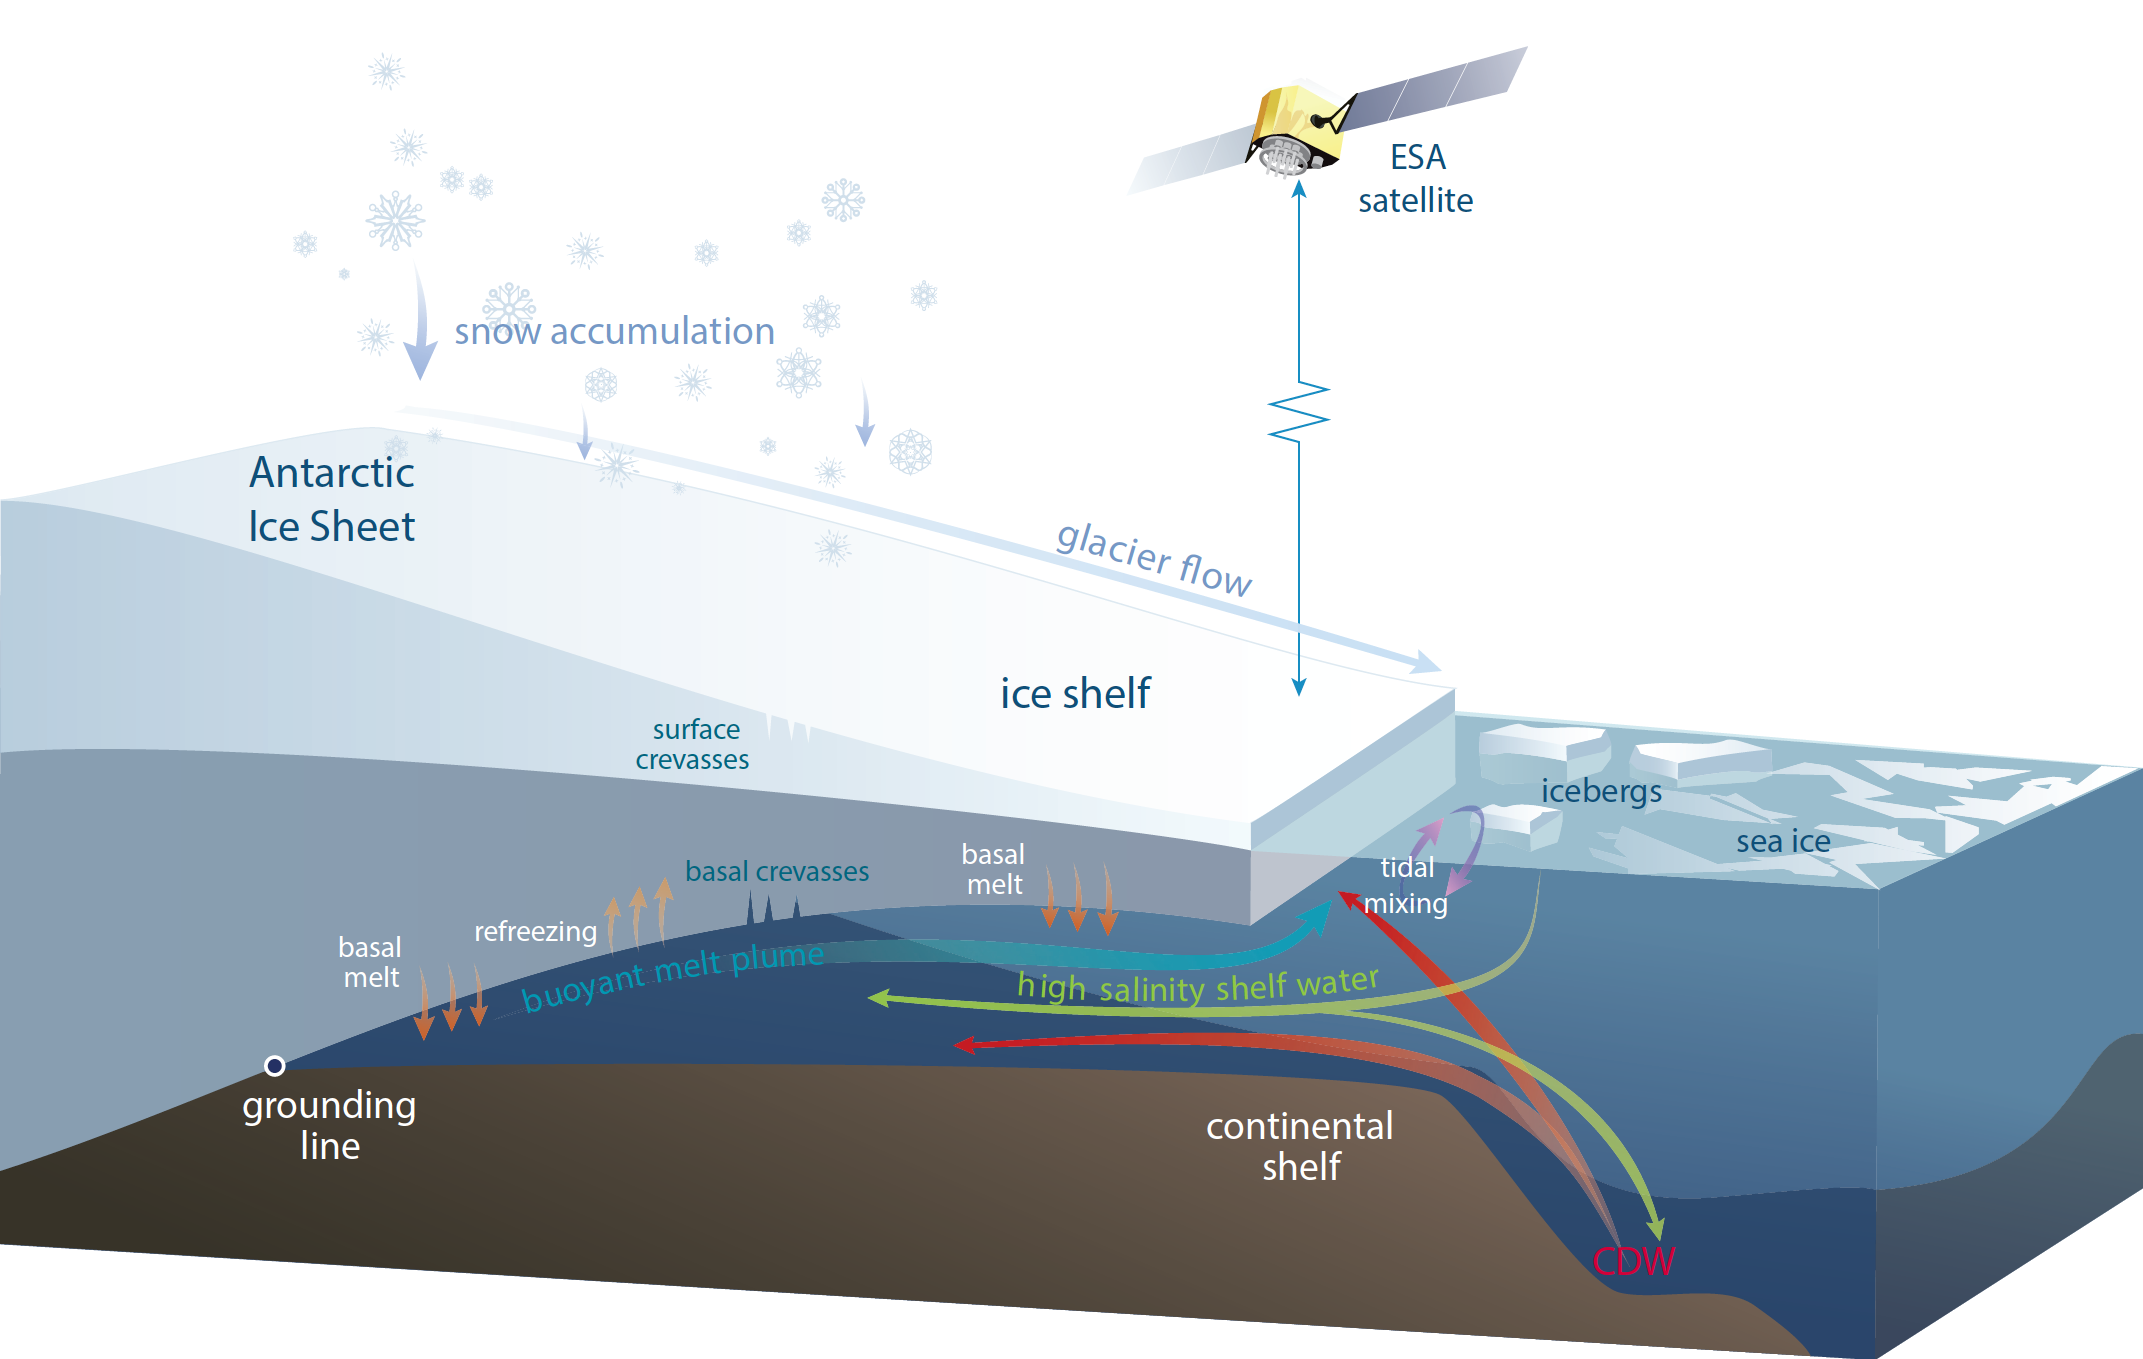
\includegraphics[width=.9\textwidth]{img/ice_shelf_diagram.png}
  \caption[Schematic of ice-shelf/ocean interaction]{
Schematic of an Antarctic ice shelf showing the primary processes causing ice-shelf volume changes. Ice is added to the ice shelf by glaciers flowing off the continent and by local snowfall that compresses to form additional ice. Ice is lost when icebergs break off the ice front, and by melting at the ice base in some regions as warm water flows into the ocean cavity under the ice shelf. Under some ice shelves, cold and fresh meltwater rises to a point where it refreezes onto the ice shelf. In this schematic, the grounding line is sitting on a ``retrograde'' slope (sloping down-wards towards the continental interior).
  }
  \label{fig:ice-shelf-schematic}
\end{figure}


In essence, since the grounded ice sheet changes in response to perturbations in the ice
shelves, understanding variations in the state of the ice shelves is key to
identifying relationships between observed ice loss and large-scale climate variability.
There are two complementary ways forward: to develop our understanding of the actual mass
loss processes, so they can be better represented in models; and to empirically relate observed
ice-sheet change to ocean and atmospheric variability. This dissertation focuses on the second
approach.

\section{Satellite altimetry and ice-shelf change detection}

\noindent
Continuous observations of ice shelves over long periods of time are required to determine their stability,
monitor change, and identify general relationships between observed changes and ocean
variability. Given the vast size of Antarctica, its remote location and challenging field conditions,
space-based techniques are the only practical way to monitor the ice shelves.
Much of our current understanding of how ice-shelf processes couple ice-sheet changes to climate variability comes from analyses of trends in surface elevation change, $\del h / \del t$, derived from satellite radar and laser altimeter measurements (Fig.~\ref{fig:ice-shelf-schematic}) \parencite{Zwally2005, Shepherd2010, Pritchard2012, Fricker2012}.
In particular, satellite radar altimeters
have provided the longest set of continuous observations over the Antarctic and Greenland ice sheets, and have dramatically changed our ability to study these ice masses. Maps of ice-shelf height change at high spatial resolution have also been developed using measurements from a satellite laser altimeter (ICESat)\footnote{ICESat (Ice, Cloud, and land Elevation Satellite), was a NASA satellite mission for measuring ice sheet mass balance, cloud and aerosol heights, as well as land topography and vegetation characteristics. It operated from 2003 to 2010.} \parencite{Pritchard2012}, but the time span of the data set only covered the period 2003--2008 (5 years). In contrast, satellite radar altimeters have been providing
measurements of the ice shelves since 1978\footnote{Although another radar altimeter flew before
this date over the ice sheets (the GEOS-3), its experimental measurements were not
useful for ice-sheet change determination.} \parencite{Zwally1983, Zwally1989, Davis1998, Martin1983}. However,
historical RA missions like Seasat (1978) and Geosat (1985--1989) were limited to orbit latitudes north of 72\degree S (south of 72\degree N for Greenland) and, although insufficient for whole ice sheet studies, this coverage did capture a portion of the fringing ice shelves and marginal grounded ice \parencite[e.g.,][]{Fricker2012}.

More than two decades of modern (global) RA missions,
including ERS-1 (1992--1996), ERS-2 (1995--2003), Envisat (2002--2012), and Cryosat-2 (2010--present), have dramatically improved our understanding of ice-sheet
mass balance and its relation to measured sea-level rise \parencite[e.g.,][]{Shepherd2012, Wingham2006}. In general, however,
studies focusing on the ice shelves using RA have under-exploited these data,
reporting linear height-trends for a fraction---and usually for broad regions---of the complete (modern-era) RA data set \parencite[e.g.,][]{Shepherd2003, Shepherd2010, Zwally2005}.

A satellite radar altimeter measures the satellite-to-surface round-trip travel time of the emitted electromagnetic waves (Fig.~\ref{fig:ra-principle}). The standard altimeters used in this study operated in the Ku-band (microwaves): 13.6--13.8 GHz frequency, 2.2--2.3 cm wavelength. As electromagnetic waves travel through the atmosphere, they can be delayed by water vapour or by ionization. Once these effects are corrected for, the final range $R$ is estimated with high precision\footnote{The strength of satellite radar altimeters is their single-measurement high precision, which is fundamental for estimating changes (more so than accuracy).}. The radar-altimeter's response over ice surfaces is considerably more complex than over the oceans. Causal factors identified in the complex backscatter response over ice sheets include: sloping surfaces, surface undulations with characteristic wavelengths on the same spatial scale as the altimeter beam-limited footprint, off-track reflections, dynamic lag of the altimeter tracking circuit (on-board, which requires off-board post-processing---\emph{retracking}), and spatio-temporal variations in the ice-surface properties (leading to backscatter fluctuations) \parencite{Martin1983}. %\emph{Retracking} methods using the altimeter return-pulse waveforms (Fig.~\ref{ch1figX}) give range corrections that are typically several meters, and significant differences are found between different \emph{retracking} algorithms \parencite{Davis1996}.


\begin{figure}[!ht]
  \centering
  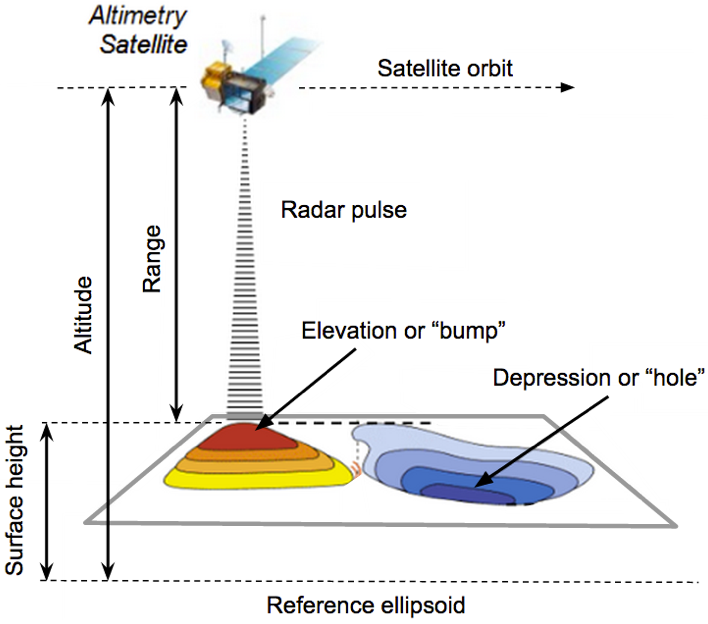
\includegraphics[width=.75\textwidth]{img/altimetry_principle.png} \\[.5cm]
  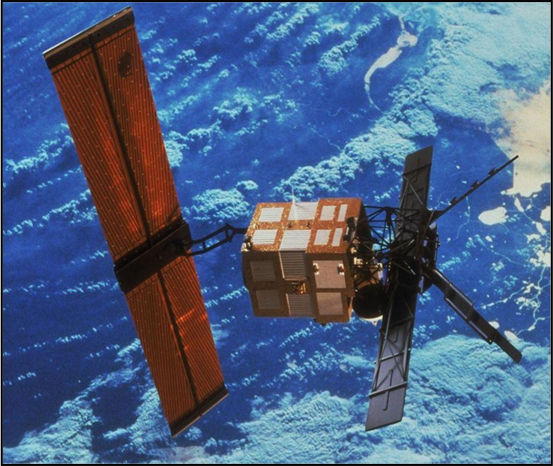
\includegraphics[height=4.2cm]{img/ers1.png}
  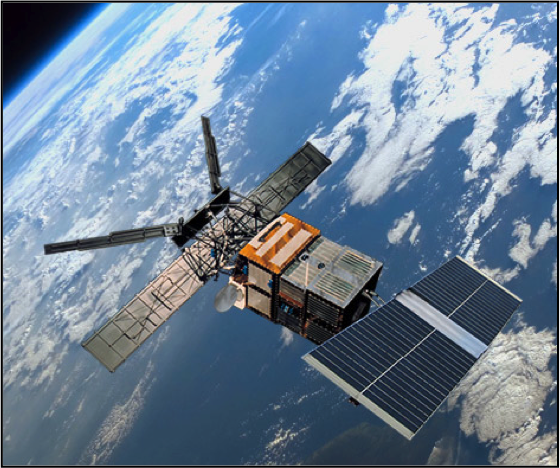
\includegraphics[height=4.2cm]{img/ers2.png}
  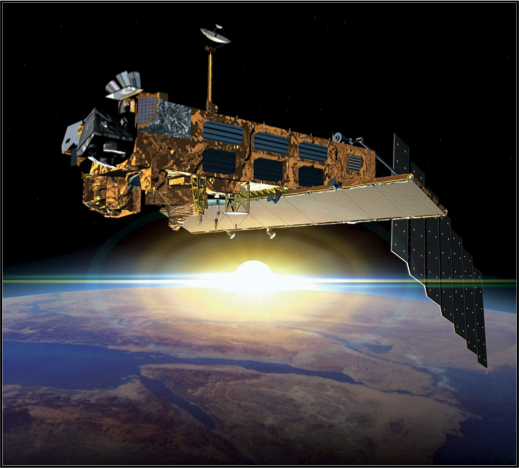
\includegraphics[height=4.2cm]{img/envisat.png}
  \caption[Measurement principle of satellite radar altimetry]{
  Measurement principle of a satellite radar altimetry. (top) Radar altimeters estimate the height of surface reflectors (with respect to a reference ellipsoid, e.g., WGS84) by measuring the satellite-to-surface round-trip travel time of radar pulses. (bottom) The three European Space Agency satellites used in this study (from left to right): the European Remote Sensing Satellite-1 (ERS-1, 1992--1996), the European Remote Sensing Satellite-2 (ERS-2, 1995--2003), and the Environmental Satellite (Envisat, 2003--2012).
  }
  \label{fig:ra-principle}
\end{figure}
\clearpage

\newpage

The ice-shelf height measured by an altimeter can be represented as:

\begin{equation}
  h = A - R - D
\end{equation}
\label{eq:ra-height}

\noindent
where $h$ is the surface height with respect to the ellipsoid, $A$ is the satellite's altitude, $R$ is the satellite-to-surface measured range, and $D$ represents the atmospheric path delay (accounted for) (Fig.~\ref{fig:ra-principle}). $h$ is derived, along with other parameters, from the radar echo waveform (or shape of the return pulse; Fig.~\ref{fig:ra-footprint-waveform}). By performing repeated measurements over time we can track changes in the ice-shelf height, that relates to the ice-shelf mass balance as follows:

\begin{equation}
\begin{split}
  \frac{\del h}{\del t} &= 
    \overbrace{
      \frac{\del \Delta}{\del t}
      \rule[20pt]{0pt}{5pt}}^{\mbox{a}}
    -\overbrace{
      M \, \frac{\del}{\del t} \, \rho^{-1}_\text{w}
      \rule[20pt]{0pt}{5pt}}^{\mbox{b}}
    +\overbrace{
      \int^M_0 \text{d}m \, \frac{\del}{\del t} \, \rho^{-1}_\text{f}(m)
      \rule[20pt]{0pt}{5pt}}^{\mbox{c}} \\
    &\quad +\underbrace{
      ( \, \rho^{-1}_\text{i} - \rho^{-1}_\text{w} \, ) 
      \rule[-11pt]{0pt}{5pt}}_{\mbox{d}}
    \cdot \, ( \, 
      \underbrace{ \dot{M}_\text{s} + \dot{M}_\text{b}
      \rule[-11pt]{0pt}{5pt}}_{\mbox{e}}
      + \, 
      \underbrace{ \vect{u} \cdot \nabla M + M \nabla \cdot \vect{u} 
      \rule[-11pt]{0pt}{5pt}}_{\mbox{f}}
    \, )
\end{split}
\end{equation}
\label{eq:ra-height-change}

\noindent
where $\Delta$ is ocean-surface level; $M$ is ice/water mass; $\rho_\text{w}$, $\rho_\text{f}$ and $\rho_\text{i}$ are density of water, firn and ice, respectively; and $\vect{u}$ is horizontal velocity. So that each term in the equation represents (a) sea-level variations, (b) ocean density changes, (c) firn compaction (air loss), (d) ice-ocean density contrast, (e) surface and basal accumulation rates, respectively, and (f) advection of thickness gradient and flow divergence, respectively.

The range of estimates for the Antarctic mass budget, derived from satellite observations over the past two decades, vary widely according to the method they are based upon---for example, from
$-$250 to $+$50 Gt year$^{-1}$ for 1992--2009 \parencite{Zwally2011}. As reported in
\textcite{Zwally2011}:

\begin{quotation}
\noindent
Generally, the range of estimates in IPCC07\footnote{Fourth Assessment Report (AR4) of the Intergovernmental Panel on Climate Change (IPCC), 2007: \url{https://www.ipcc.ch/publications\_and\_data/publications\_ipcc\_fourth\_assessment\_report\_synthesis\_report.htm}.} encompassed the errors listed in the studies, but as noted in the report, a mid-range value does not indicate a more reliable estimate, and the composite errors listed in each study do not define confidence limits because important components lack formal statistical derivation. This caution on the error estimates applies to all studies regardless of methods of data collection and analyses.
\end{quotation}

This highlights the need to account for uncertainties more consistently, as well as analyzing the inherently noisy and complex altimeter-measurements within a robust statistical framework.


\begin{figure}[!ht]
  \centering
  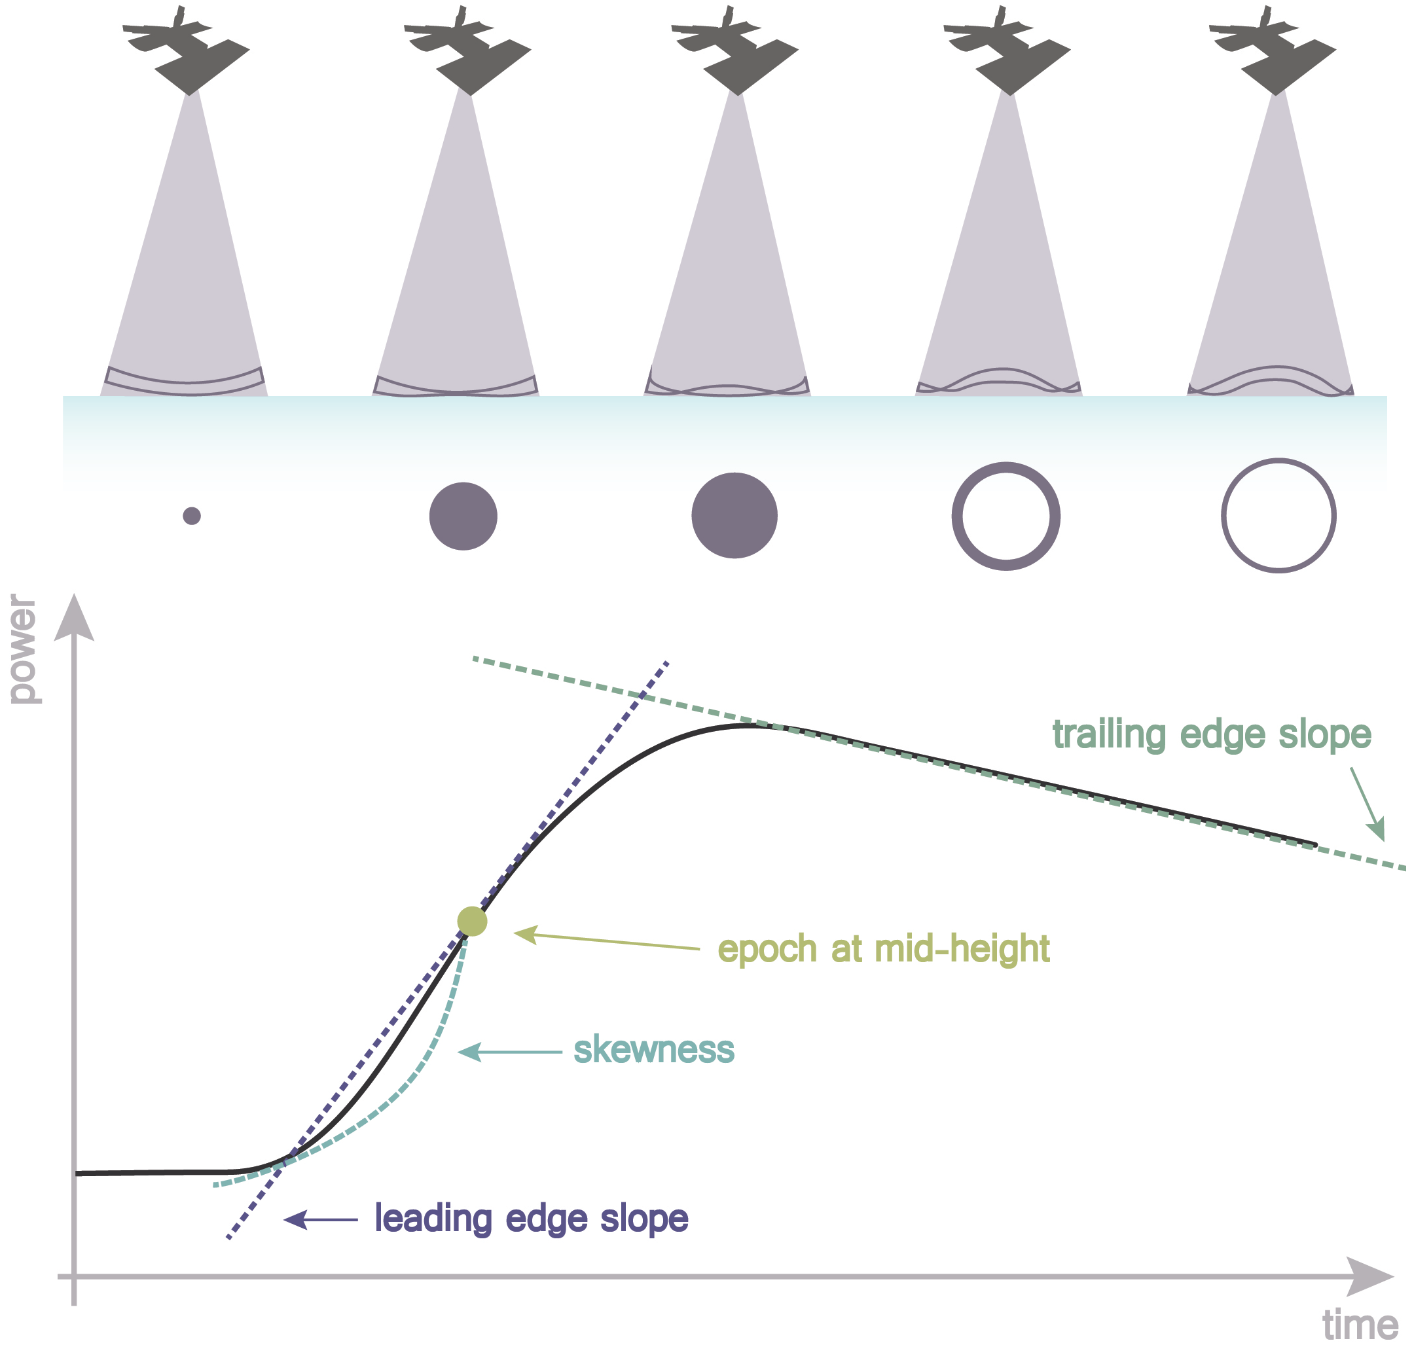
\includegraphics[width=.82\textwidth]{img/altimetry_footprint.png}
  \caption[Radar altimeter footprint and waveform]{
Radar altimeter footprint and waveform. (top) The radar altimeter receives the reflected wave (or echo), which varies in intensity over time. Over a flat surface the reflected wave's amplitude increases sharply from the moment the leading edge of the radar signal strikes the surface. (bottom) The echo waveform has a characteristic shape that can be described analytically (the Brown model). From this shape, several parameters can be deduced by comparing the real (averaged) waveform with the theoretical curve. \emph{Epoch at mid-height}: this gives the time delay of the expected return of the radar pulse (estimated by the tracker algorithm) and thus the time that the radar pulse took to travel the satellite-surface distance (\emph{Range}) and back again. \emph{Amplitude of the useful signal}: this amplitude with respect to the emission amplitude gives the backscatter coefficient ($\sigma_0$). \emph{Thermal noise}: the instrument's (internal) background noise. \emph{Leading-edge slope}: this can be related to the significant wave height (SWH). \emph{Skewness}: the leading edge curvature. \emph{Trailing-edge slope}: this is linked to any mispointing of the radar antenna (any deviation from nadir of the radar pointing). {\it Credit: modified from ESA's Radar Altimetry Tutorial; Caroline Fleet}.
  }
  \label{fig:ra-footprint-waveform}
\end{figure}


\section{Scientific objectives}

\noindent
This dissertation seeks to address the following scientific questions.
a) Has $\del h / \del t$ for Antarctic ice shelves been constant
or has it varied over time?
b) Are the observed changes restricted to particular regions or do they
occur in a larger scale?
c) What are the spatial patterns of coherence in $\del h / \del t$
around Antarctica?
d) Are there links between interannual variations in the ice shelves and
large-scale climate variability?

To answer these questions we designed this PhD research around three main objectives, which became chapters of this dissertation:

\begin{enumerate}
  \item[i.] {\it Derive reliable time series of height change} ({\sl Chapter 2}). Improve and
  extend the procedures for extracting height changes from multi-mission RA
  records, deriving reliable long-term, continuous time series in a
  high-resolution grid for consistent trend and variability analysis.
  \item[ii.] {\it Quantify long-term trends} ({\sl Chapter 3}). Analyze long-term changes for
  all Antarctic ice shelves spanning a time period of nearly two decades,
  mapping in time and space the rate of change in ice-shelf height and volume, the acceleration
  and associated uncertainties.
  \item[iii.] {\it Analyze interannual variability} ({\sl Chapter 4}). Use the
  extended time series and spatial maps to seek relationships between
  fluctuations in ice-shelf height and known modes of variability in the
  atmosphere and the ocean (such as El Ni\~{n}o-Southern Oscillation).
\end{enumerate}

\clearpage

\section{Summary of results}

\noindent
This dissertation presents methods for improved analysis of ice-shelf height data from multiple satellite RAs and estimation of uncertainties in the resulting products. We constructed 18-year-long time series of height changes at $\sim$3 month intervals and $\sim$30 km grid cells over Antarctica's floating ice shelves. Our data set allowed us to estimate, reliably, the temporal progression and spatial structure of changes in ice-shelf height in Antarctica between 1994 and 2012.

We have demonstrated that: i) substantial averaging both in time and space is required to
construct reliable RA height records over floating ice shelves; ii) densification of the surface
strongly affects the height-change estimate, and the backscatter correction significantly reduces
this effect; iii) densification is a more important effect than penetration in biasing the height-change
estimates over the ice shelves; iv) given the high interannual-to-decadal variability that is present, a
simple straight-line fit fails to capture the underlying trends, some degree of curvature in the
trend is needed; v) polynomial trends allow us to obtain information on the evolution and spatial
structure of changes, for instance, instantaneous rate of change (derivative of the trend) and average
acceleration (slope of the derivative); and vi) given the convoluted nature of the error sources, we
propose that a top-down approach for uncertainty estimation (such as bootstrap applied to time-dependent data) constitutes a more accurate alternative for error analysis.

We have shown that Antarctic ice-shelf volume
loss is accelerating. In the Amundsen Sea,
some ice shelves buttressing regions of grounded
ice that are prone to instability have experienced
sustained rapid thinning for almost two decades.
If the present climate forcing is sustained, we
expect a drastic reduction in volume of the rapidly
thinning ice shelves at decadal to century
time scales, resulting in grounding-line retreat
and potential ice-shelf collapse. Both of these processes
further accelerate the loss of buttressing,
with consequent increase of grounded-ice
discharge and sea-level rise. On smaller scales,
ice-shelf thickness variability is complex, demonstrating
that results from single satellite missions
with typical durations of a few years are
insufficient to draw conclusions about the long-term
response of ice shelves. Large changes occur
over a wide range of time scales, with rapid variations
of ice-shelf thickness suggesting that ice
shelves can respond quickly to changes in oceanic
and atmospheric conditions.

We have presented a signal-detection procedure that (a) optimizes the fundamental signal-to-noise ratio problem through the combination of multivariate singular spectrum analysis, principal component analysis, maximum entropy and multi-taper methods; and (b) tests assumptions regarding the detectability of signals immersed in background noise, which is of fundamental importance in analyzing short and noisy records. We have shown that there is significant variability in ice-shelf height in the AS sector, particularly at the interannual scale. This interannual response is strongly correlated with the low-frequency mode of El Ni\~no-Southern Oscillation (ENSO). Due to the convoluted nature of different modes of variability and lack of observations, an ENSO signature in Antarctica has been suggested but not unequivocally demonstrated so far. Thus, our results are the first direct observational evidence of a teleconnection between climate dynamics in the tropical Pacific Ocean and the mass balance of Antarctic ice shelves and, through the buttressing effect, the Antarctic Ice Sheet. This may ultimately allow us to improve our models for predicting future ice loss.

\section{Future research}

\noindent
Our variability analysis performed on the 18-year record of ice-shelf height changes in the Amundsen region, showed that there is significant interannual fluctuation in Antarctic ice-shelf volume. This variation in ice-shelf mass not only fingerprints the mechanisms by which oceanic and atmospheric forcing perturbs the ice-sheet flow, but also provides the basis for estimating changes in freshwater fluxes around Antarctica (an important and poorly constrained parameter for modeling the polar-ocean circulation and ice-sheet dynamics). As the subject of a planned postdoctoral project, we will focus on two complementary analyses based on the results and products presented in this dissertation. 1) We will extend our study on the ENSO-Amundsen linkage by including potential correlations of estimated ice-shelf ``modes'' of variability with other climatic variables such as sea-ice extent, wind velocity and sea-surface pressure off the coast of Antarctica. 2) We will convert our regional estimates of ice-shelf volume changes to equivalent ``excess'' freshwater flux to estimate and map the time-dependence of freshwater input to Antarctic coastal regions (Ross, Amundsen, Bellingshausen, Larsen, Filchner-Ronne, Queen Maud, Amery, and Wilkes) previously defined by \textcite{Paolo2015}. 
